\documentclass[10pt]{article}
\usepackage{geometry}
\geometry{letterpaper}
\usepackage{graphicx}
\usepackage{amssymb}
\usepackage{epstopdf}
\usepackage{setspace}
\usepackage{hyperref}
\usepackage{subfig}
\usepackage{multirow}
\DeclareGraphicsRule{.tif}{png}{.png}{`convert #1 `dirname #1`/`basename #1 .tif`.png}
\graphicspath{{../../../../analysis/graphs/}}

% Set citation style
\usepackage{natbib}
\bibpunct{(}{)}{;}{a}{,}{}

\title{A Comparison of Network Diffusion and Text Regression Models for Estimating Political Ideology: Congressional Twitter Data}
\author{Drew Conway and John Myles White}
\date{\today}

\begin{document}
\maketitle

\section{Introduction}
Within the social sciences, interest in statistical methods for the automatic analysis of text has grown considerably in recent years.  Specifically, within the field of political science there has been continued interest in using text analysis to extend well-known spatial models of political ideology \citep{Grimmer_2011, Monroe_2008, Laver_2003}.  Moreover, interest in how the structure of social networks affects political attitudes and outcomes has been both growing \citep{Siegel_2009, Burton_2009} and controversial \citep{Fowler_2010, Lyons_2010}.  In an attempt to bridge the gap between these two research areas we have collected a large sample of Twitter data related to the U.S. Congress. Twitter provides a rich data set containing both text and social network information about its members. Here we compare the usefulness of text analysis and social network analysis for predicting the political ideology of Twitter users --- two methods that are, in principle, applicable to both members of Congress (for whom roll call data and precise spatial estimates of political ideology already exist) and to the surrounding network of Twitter users (for whom precise estimates of political ideology do not exist). To compare text analysis methods with tools from social network analysis, we fit a variety of L1- and L2-regularized regression models that use word count data from individual tweets to predict the ideal points of members of Congress. We then compare the performance of the resulting text models with the performance of social network models that employ techniques developed to model diffusion over networked structures to estimate the ideal points for the same members of Congress. In this preliminary study we find that each method provides novel insight into the ideological spectrum of the U.S. Congress.

\section{Methods}
Using data from the Sunlight Foundation, we have identified 67 Senators and 313 Representatives who maintain a presence on Twitter.\footnote{The Sunlight Foundation provides this information via its API at \url{http://services.sunlightlabs.com/docs/Sunlight_Congress_API/}.} For these members of Congress, we have generated a data set of nearly one-hundred thousand tweets posted to Twitter between the period of November 11, 2007 and August 15, 2011.  The data were harvested using a spider written in Python that makes calls to Twitter's API on a regular basis.\footnote{The code used to generate this corpus, and all other data related to this project, can be inspected and downloaded here: \url{https://github.com/drewconway/Twitter-Congress}.  Readers should note, however, that due to Twitter's data policies the raw data set of tweets could not be shared.  Also, due to the moving window of data available in Twitter's search API any replication of the data using the code available here may not match exactly what is used in this following analysis.}  Each tweet in the data set contains the following information: full name of member of Congress, title (Senator or Representative), party affiliation, home state, gender, Twitter user name, text of tweet, date and time the tweet was published, and the unique ID number for the tweet within Twitter's database.

In addition to this source of text data, we have used Google's SocialGraph API to generate the directed social graph for the members of Congress who use Twitter.\footnote{We have used Google's social graph service rather than Twitter's because our need to build the full social graph of all members of Congress exceeded the limits provided by the Twitter API, but was within Google's.} Summary statistics for this graph are shown in Table 1.

\begin{table}[htdp]
    \centering
    \caption{Summary Statistics for Main Component of Congressional Twitter Network}
    \begin{tabular}{|c|c|c|c|c|}
        \hline
        Nodes & Edges & Density & Mean Degree \\ \hline
        418,941 & 926,385 & 2.21 & $5.28e^{-6}$ \\ \hline
    \end{tabular}
\end{table}

Taken together, the text and social network data set provides a useful testbed for comparing methods for measuring political ideology. Because we can use ideal points measured for all of the members of Congress based on roll call data \citep{Jackman_2001}, it is possible to test our predictions rigorously. And the bicameral nature of the Congress provides a natural division for testing a predictive model on held out data: we fit our models to data from the House and then test the models on data from the Senate.

Given both text data and social network data, there are two obvious models that we can fit: a text regression model in which the word counts for each tweet are used to predict the ideal point of the tweeting member of Congress and a social network model in which structural position is indicative of ideological position.  In this case we can model this process as a diffusion of ideological broadcasts through the social network with a given rate of absorption and decay at each node. By comparing the RMSE of both models on data from the Senate after fitting the models to the House, we can determine the viability of both analytic methods.

\subsection{Text Regression}

The 96,829 tweets in our data set can be treated as 96,829 separate observations; for each of these tweets, we observe the number of occurrences of any of the 40,000+ words in our corpus of tweets. Because many words occur only once, we have removed the terms that occur in less than 90 documents. After pruning, we have only 1,361 terms. Given the measured word counts as a predictor matrix, we attempt to predict the ideal point of the member of Congress that wrote each tweet in a standard linear regression with either L1 and L2 regularization of the fitted coefficients. Additionally, we perform regressions using either (a) only the hashtags mentioned in tweets or (b) only the mentions of other Twitter users occurring in our tweets. Results from all four regressions are reported below.

We fit the model using standard convex optimization techniques: this is implemented in the R package, \texttt{glmnet}, which we have used for our analyses. Using this software, we fit several model variants, including two L1-regularized models that use only the hashtags and mentions from the tweets. Even these substantially impoverished models (there are only 79 hashtags and 27 mentions) outperform the baseline model on held out data.

\subsection{Network Model} % (fold)
To model political ideology on the Congressional network we construct a simple model of transmission using linear decay.  We use the Jackman scores as assumed ideal points for one set of members of Congress, i.e., either Representative or Senators.  These scores are then `broadcast' over the network, and each node absorbs this score at a linear rate of decay based on geodesic distance from the broadcasting node.  Equation 1 below describes the form of this model.

\begin{equation}
    \hat{\pi_{v}} = \displaystyle\sum_{i=1}^{N} \frac{\pi_{i}}{k+1}
\end{equation}

This equation states that the estimated ideology of some node, $\hat{\pi_{v}}$, is equal to the sum of all broadcast ideologies for some set $N$ of nodes within the network.  In the case of the Congressional Twitter network, the set $N$ will either be the set of Representative or Senators.  These ideological broadcasts decay at an linear rate given the geodesic distance $k$ of $v$ from $i$.  There have been many different decay rates proposed for information transmission in networks within the literature literature \citep{Wu_2004}.  Given the scale of the network this simple linear additive model is preferable both theoretically and for computational tractability.  

\section{Results}
The results from the text regression and network model analyses are shown in Table 2 below. For the text regression, the baseline model uses only the average ideal point to make predictions for Senators, while the L1 and L2 regularized regression models use coefficients for all 1,361 terms in our pruned corpus. The Hashtags Only model is an L1 regularized regression model using a subset of 79 of the predictors from the full L1 model; similarly, the Mentions Only model is an L1 regularized regression model using only 27 of the predictors from the full L1 model. As an example of the terms that are given large weights by our regression models, we have shown the ten hashtags and mentions with the largest weights: these terms represent either the most strongly Republican or most strongly Democratic terms in our corpus.

With the network model, we see that the results are slightly better than from the text model.  For the results reported in Table 2, we use the ideological scores for the opposing house to predict the other.  For example, we use the scores for the House of Representatives to predict the ideology of Senators in the Twitter network.  As you can see from the table the model for the Senate performs quite well, explaining about 26\% of the variance between the baseline and model RMSE.\footnote{A simple linear transformation was done to the raw network model scores to scale them with respect to the Jackman scores.}

\begin{table}
    \centering
    \caption{Comparison of text regression and network models}
    \begin{tabular}{llll}
        \hline
        & Model & RMSE & $R^{2}$ \\ \hline
        \emph{Text Regression} & & & \\
        & Baseline Model & 1.062 & \\
        & L1 Regularization & 0.9729 & 0.08390 \\
        & L2 Regularization & 0.9771 & 0.07994 \\
        & Hashtags Only & 1.037 & 0.02354 \\
        & Mentions Only & 1.058 & 0.00377 \\ \hline
        \emph{Network Model} & & & \\
        & Sen. Baseline & 1.010 & \\
        & Sen. Estimate & 0.7470 & 0.26097 \\
        & Rep. Base & 0.9949 & \\
        & Rep. Estimates & 0.8577 & 0.1378 \\ \hline
    \end{tabular}
\end{table}

\begin{table}[!ht]
    \caption{Top 5 Republican and Democratic Hashtags and Mentions from Lasso}
    \centering
    \begin{tabular}{cr|l||r|l}
        & Hashtag & Weight & Mention & Weight \\
        \hline
        \multirow{5}{*}{\emph{Republican}}
        & \#jobs & 1.0288 & @speakerboehner & 0.7664 \\
        & \#p2 & 0.6820 & @foxbusiness & 0.7126 \\
        & \#dadt & 0.6780 & @foxnews & 0.6955 \\
        & \#reins & 0.6307 & @gopwhip & 0.6776 \\
        & \#tx17 & 0.6292 & @thehill & 0.6505 \\
        \hline
        \multirow{5}{*}{\emph{Democrat}}
        & \#askobama & -1.2113 & @cspan & -0.0743 \\
        & \#pa11 & -1.2181 & @wsj & -0.1875 \\
        & \#debt & -1.2209 & @rephensarling & -0.2954 \\
        & \#healthcare & -1.3877 & @natresources & -0.5474 \\
        & \#libya & -1.6383 & @barackobama & -1.1266 \\
        \hline
        \end{tabular}
\end{table}

In Figure 1 we visualize the relationship between the baseline Senate scores and the predicted ones from the model.  In the right panel of Figure 1 we replace the points with the surnames of the senators.

\begin{figure}[!ht]
    \centering
    \subfloat[Ideal Points]{\label{fig:points}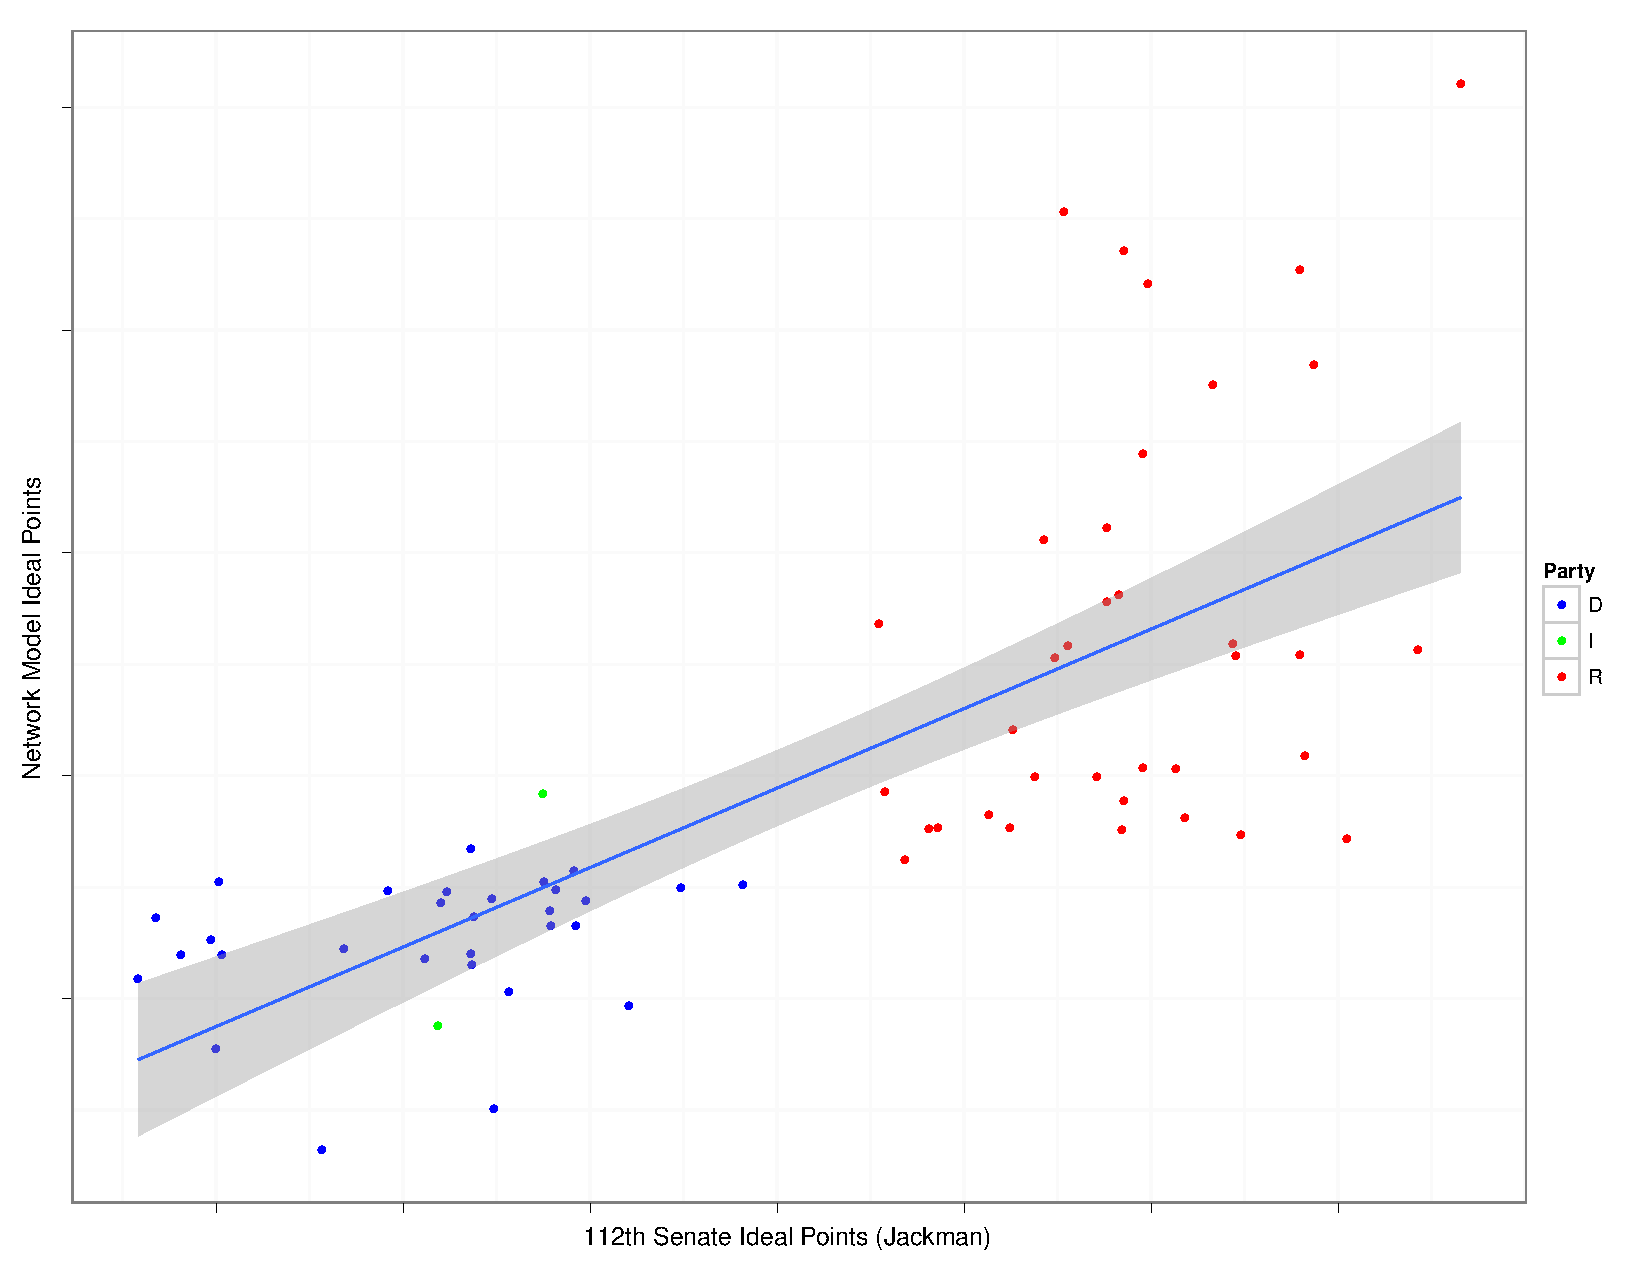
\includegraphics[width=.5\textwidth]{sen_pts.pdf}}
    \subfloat[With Sen. Surnames]{\label{fig:points}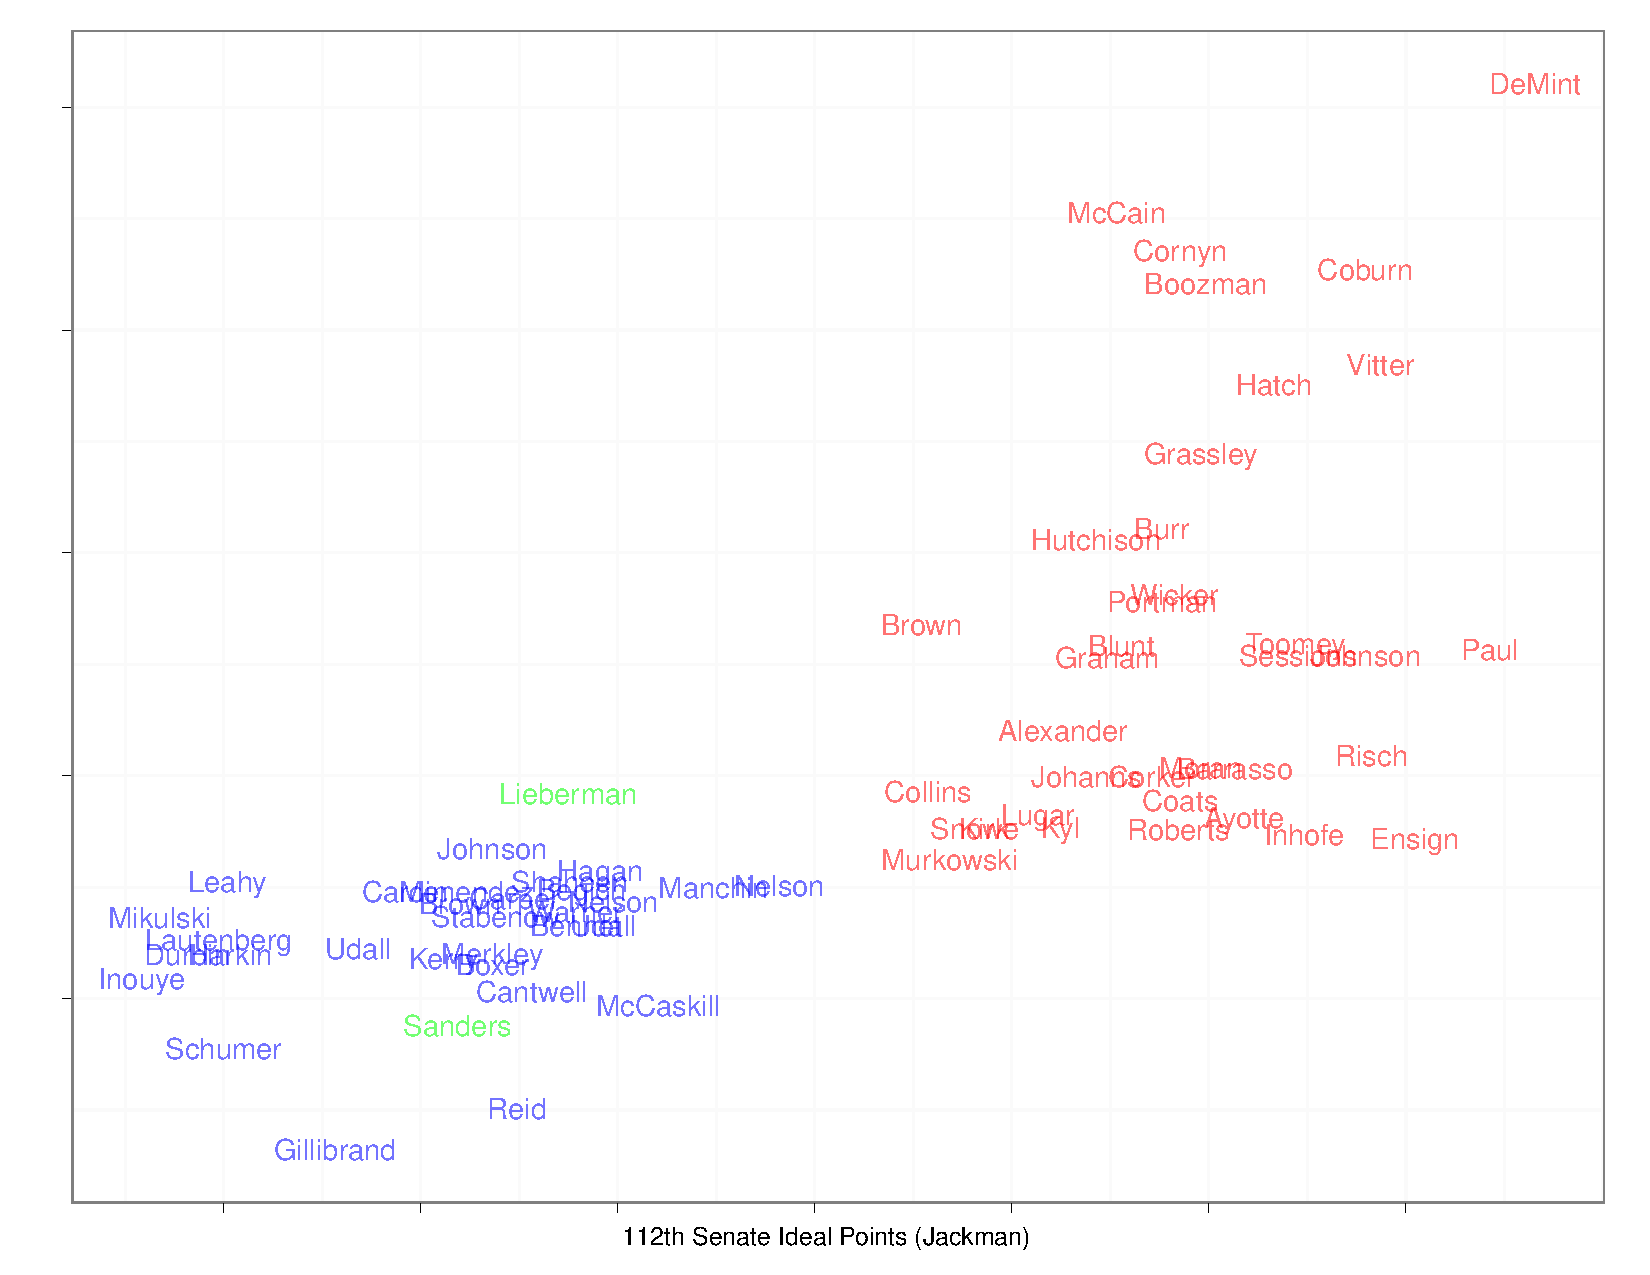
\includegraphics[width=.5\textwidth]{sen_names.pdf}}
    \caption{Fit of Network Model Results for Senators}
    \label{fig:senators}
\end{figure}

\section{Discussion}
Our work provides a proof of concept demonstration of the viability of using both social network and text derived from Twitter to model the political culture of the U.S. Future work will need to improve on the fine details of the methods we have employed. Another promising research project is to construct statistical models that employ social network and text data simultaneously as a twofold set of constraints for the estimation of spatial models of political ideology.

For the network model, we are not concerned with the context of a member of Congress's tweets, but rather how they are position within the greater social network of Twitter exposes their political ideology.  This is particularly interesting because Twitter is a \emph{directed graph}, meaning that relationships are not mutual.  The model, therefore, shows that given a set of fixed ideological broadcast nodes within the structure of Twitter, we can accurately estimate the ideology of all other nodes regardless of whether they actually follow anyone.  Put another way, who follows you on Twitter tells us as much about your ideology as who you follow.

\bibliographystyle{chicago}
\setstretch{1.0}
\bibliography{abs} 

\end{document}
